\section{DeepProbLog}
\label{sec:DeepProbLog}

\begin{figure*}[ht]
\centerline{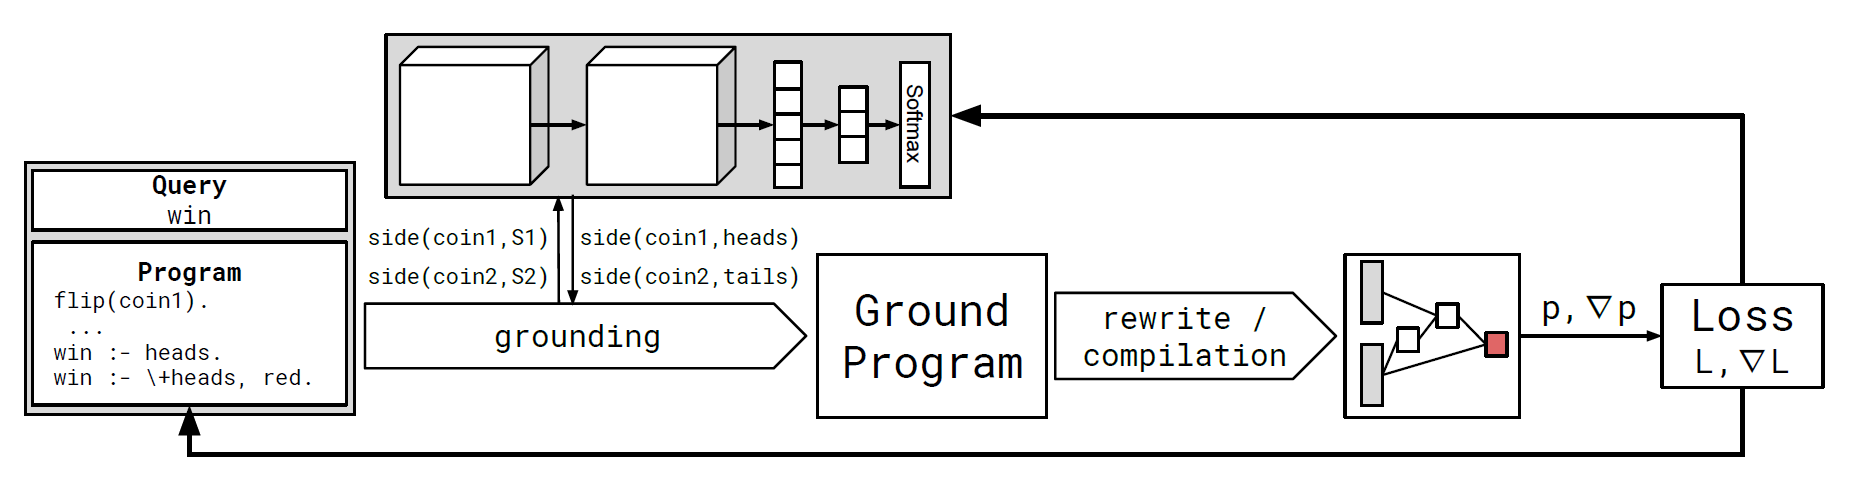
\includegraphics[scale=0.4]{learning_pipeline.png}}
\caption{The learning pipeline \cite{ProbLog}.}
\label{fig:learning_pipeline}
\end{figure*}


In this section, we explain briefly the basics of probabilistic logic programming using ProbLog and how to extend it to obtain DeepProbLog.

A ProbLog program is made of a set of ground probabilistic facts $\mathcal{F}$ of the form $p :: f$ where $p$ is a probability and $f$ is a ground atom, and a set of rules $\mathcal{R}$.
One extension introduced for convenience that is nothing else than syntactic sugar are the annotated disjunctions (ADs). An annotated disjunction is an expression of the form 
\begin{equation}
\label{eq:ad}
    p_1 :: h_1 ; \dots ; p_n :: h_n {:-} b_1, \dots, b_m.
\end{equation}
where the $p_i$ are probabilities that sum to at most one, the $h_i$ are atoms and the $b_j$ are literals. Given the AD of Eq. \ref{eq:ad}, when all $b_i$ hold then one of the heads $h_j$ will be true with probability $p_j$ or none of them with probability $1 - \sum{p_i}$. Several of the $h_i$ may be true at the same time if they also appear as heads of other ADs or rules. Since ADs are syntactic sugar, they do not change the expressivity power of ProbLog and can be alternatively modeled as facts and logical rules \cite{DeRaedt2015}.
% ProbLog programs with annotated disjunctions can be transformed into equivalent ProbLog programs
% without annotated disjunctions (TODO cf. De Raedt and Kimmig [2015]).

% Moreover, non-ground probabilistic facts can be defined in ProbLog as a shortcut to model a set of ground probabilistic facts.

% The ProbLog language has the same expressive power of Bayesian Networks and a representational mapping between the two is possible.


While in ProbLog probabilities are explicitly specified as part of probabilistic facts or ADs, in DeepProbLog probabilities are specified through neural networks.
A DeepProbLog program is a ProbLog program that is extended with a set of ground neural annotated disjunctions (nADs) of the form
\begin{equation}
    nn(m_q, \vec{t}, \vec{u}) :: q(\vec{t}, u_1); \dots; q(\vec{t}, u_n) :- b_1, \dots, b_m
\end{equation}
where $nn$ is a reserved keyword that stands for 'neural network' and $m_q$ is the identifier of the neural network model, $\vec{t} = t_1, \dots, t_k$ is a vector of ground terms representing the inputs of the neural network for predicate $q$, $\vec{u} = u_1, \dots, u_n$ is the vector of the possible output values of the neural network and $b_i$ are atoms. The NN defines a probability distribution over its output values $\vec{u}$ given the input $\vec{t}$.
% The neural network can be viewed as a discriminative classifier that determines the truth value of the fact. 
The neural network could be of any type, e.g. a recurrent or a convolutional network, but its output layer, which feeds the corresponding neural predicate, needs to be normalized.
Note that a neural AD realizes a regular AD $p_1 :: q(\vec{t}; u_1); \dots; p_n :: q(\vec{t}; u_n) :- b_1; \dots; b_m$ after a forward pass on the neural network.

\subsection{DeepProbLog inference}
Inference in DeepProbLog closely follows that in ProbLog. ProbLog inference proceeds in four steps, the first step is the grounding step, in which the logic program is grounded with respect to the query, generating all ground instances of clauses the query depends on. This step uses backward reasoning to determine which ground rules are relevant to derive the truth value of the query, and may perform additional logical simplifications that do not affect the query’s probability.

The second step rewrites the ground logic program into a formula in propositional logic that defines the truth value of the query in terms of the truth values of probabilistic facts. We can calculate the query success probability by performing weighted model counting (WMC) on this logic formula even if it is not efficient.

The third step is knowledge compilation that compiles the logic formula into a Sentential Decision Diagram (SDD, \cite{SDD_Darwiche}), a form that allows for efficient weighted model counting. SDDs are a subset of deterministic decomposable negational normal forms (d-DNNFs) and as these ones allow for polytime model counting.
% they also support polytime conjunction, dis-junction and negation while being more succinct than OBDDs (Darwiche[22]).

The fourth step transforms the SDD into an arithmetic circuit (AC). The AC has the probabilities of the probabilistic facts on the leaves and is obtained replacing the OR nodes with addition and the AND nodes by multiplication. The AC is then evaluated to calculate the WMC.

Inference in DeepProbLog works as in ProbLog, the only difference is that we need to instantiate nADs and neural facts respectively to regular ADs and probabilistic facts. During the grounding step, we obtain ground nADs and ground neural facts. The concrete parameters are determined subsequently by making a forward pass on the relevant neural network with the ground input.



\subsection{Learning in DeepProbLog}
Learning in DeepProbLog consists in jointly train the learnable parameters in the logic program, i.e. the parameters of probabilistic facts, and learnable parameters of the neural network in DeepProbLog programs.
% ProbLog, just like any other statistical relational AI model such as Markov Logic [4,23], can be trained discriminatively as well as a generatively. In the generative setting, the examples are (partial) possible worlds or interpretations, while in the discriminative setting they correspond to facts for a specific target predicate with the evidence residing in the background theory.
% The authors \cite{TODO}
DeepProbLog programs are trained in a discriminative training setting, which is called \textit{learning from entailment} \cite{Frazier}. This approach proceeds as follows: given a DeepProbLog program with parameters $X$, a set $Q$ of pairs $(q,p)$ with $q$ a query and $p$ its desired success probability, and a loss function $L$, compute:
\begin{equation}
    \argmin_{\vec{x}} \frac{1}{|Q|} \sum_{(q,p) \in Q} L(P_{X=\vec{x}}(q), p)
\end{equation}
% TODO: a slighly different equation is presented in the other paper

In contrast to the approach proposed by Gutmann et al. \cite{Gutmann}, gradient descent is used rather than EM, as this method allows for seamless integration with neural network training. It is worth noting that we can use the same AC that ProbLog uses for inference for gradient computations as well: this AC is a differentiable structure, as it is composed of addition and multiplication operations only. The framework relies on the automatic differentiation capabilities already available in ProbLog to derive the gradients. More specifically, to compute the gradient with respect to the probabilistic logic program part, it relies on Algebraic ProbLog (aProbLog \cite{aProbLog}), a generalization of the ProbLog language, and inference to arbitrary commutative semirings, including the gradient semiring \cite{gSemiring}.
An overview of the approach is shown in Figure \ref{fig:learning_pipeline}.
Given a DeepProbLog program, its neural network models, and a query used as training example, we first ground the program with respect to the query, getting the current parameters of nADs from the external models, then use the ProbLog framework to compute the loss and its gradient, and finally use these to update the parameters in the neural networks and the probabilistic program. % TODO: cut-and-paste sentence
% More specifically, to compute the gradient with respect to the probabilistic logic program part, we rely on Algebraic ProbLog (aProbLog, [Kimmig et al., 2011]), a generalization of the ProbLog language and inference to arbitrary commutative semirings, including the gradient semiring [Eisner, 2002].


% TODO: we can explain deeper if needed
% TODO: sentence to conclude section

In the following section, we present and discuss the multi-digit MNIST octal-division task and how can be solved using DeepProbLog.